\section{Task 4: Pixel Intensity Along One Row and its Correlation}

Now let's plot the intensities of row 164 of cameraman.tif. The full image is
also provided for reference.

\begin{figure}[H]
    \centering
    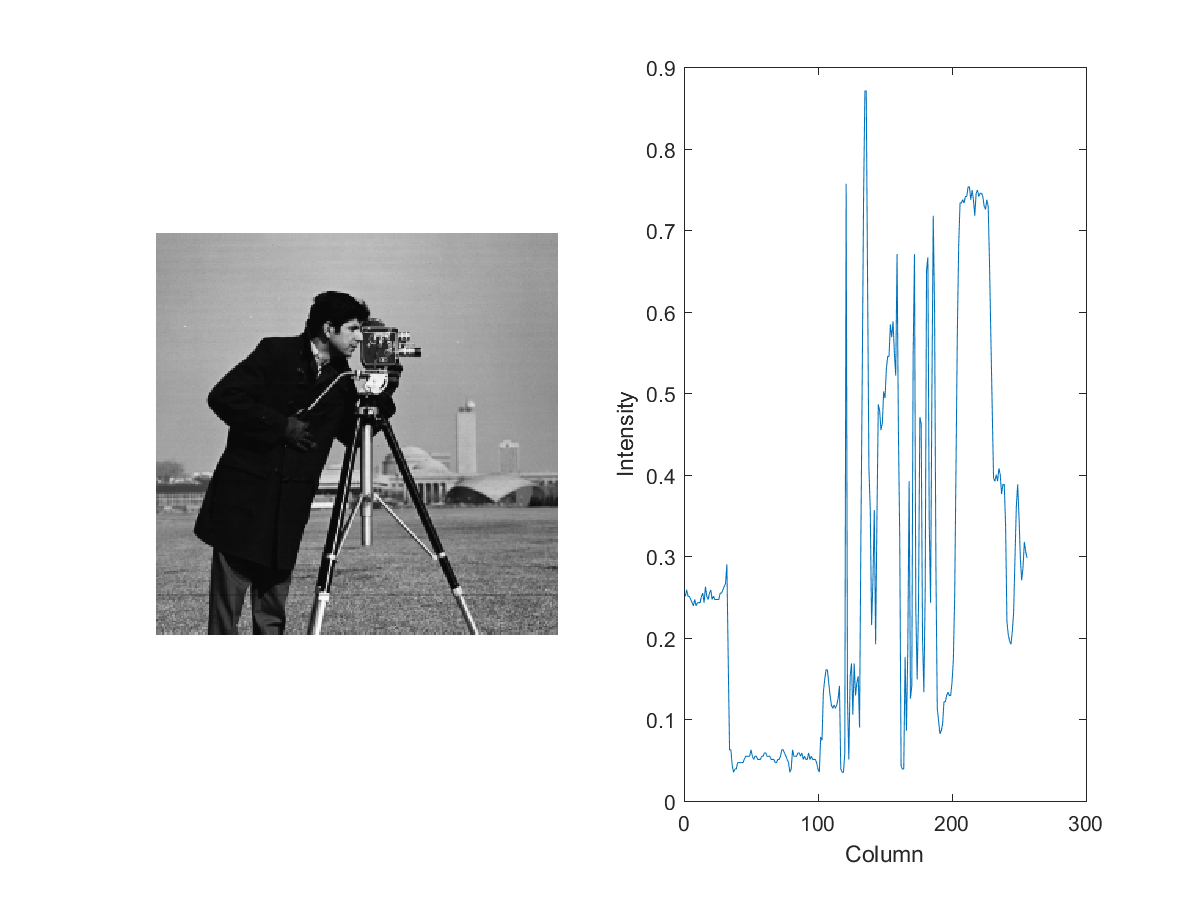
\includegraphics[scale=0.5]{rowIntensity}
    \caption{cameraman.tif and Row Intensity}
\end{figure}

There looks like there might be some correlation as we seem to be transitioning
between two intensity ranges of the foreground and background. Let's perform
autocorrelation.

\begin{figure}[H]
    \centering
    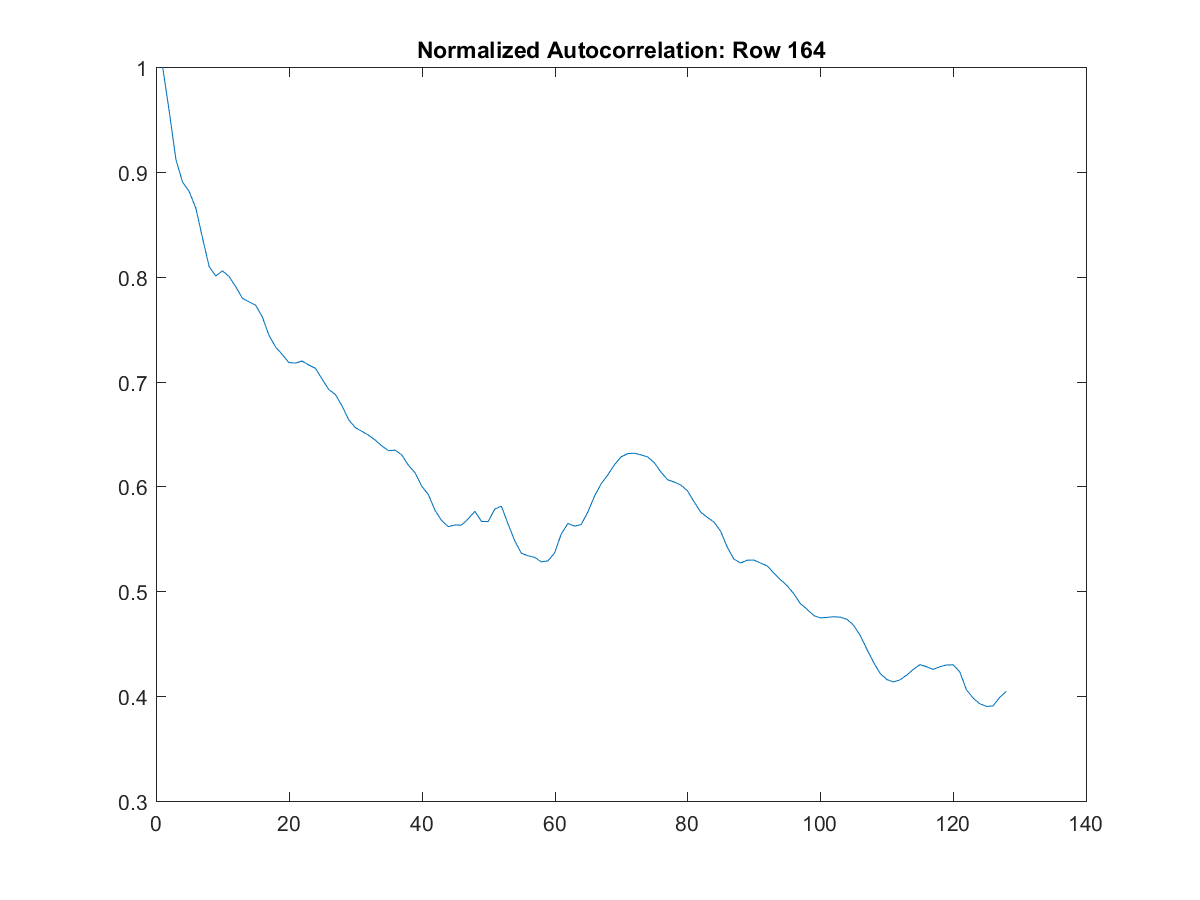
\includegraphics[scale=0.5]{autocorrelation}
    \caption{Autocorrelation of Row 164}
\end{figure}

In this case, autocorrelation starts with the signal fully overlapping itself
(and therefore correlation coefficient starts at 1). The signals are then only shifted
over half the range of the image. This is because the correlation signal would
mirror itself otherwise, and we only need to see the important information.

Continuing from earlier, we can see that there is a local peak of correlation
around column X. given the shape of this image we would likely find more
correlation in the colimns as many of the shapes are skinny and tall, and
therefore constant in value.

It is likely that many compression algorithms use correlation. If an image has a
repeating pattern, then we really only need to record that pattern once. I also
image that basic image data compression algorithms check for greater correlation
in the horizontal and vertical directions. This would account for cases where an
image is highly correlated in one direction but not the other.
